\section{Context-Aware Routing Protocols}

% \begin{figure*}[!t]
% 	\centering
% 	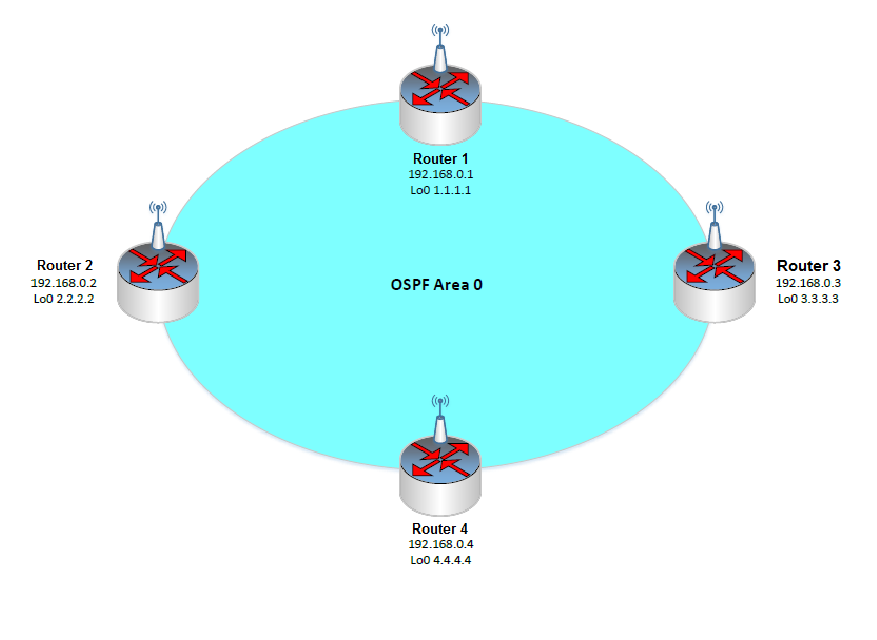
\includegraphics[width=0.7\textwidth]{figs/topology.eps}
% 	\caption{Wireless Network topology.}
% 	\label{Fig01}
% \end{figure*}

Traditional mesh routing solutions have focused on simply finding the best route to the gateway to reach the Internet. Two important underlying assumptions of these routing solutions are: 1) all gateway nodes are equally capable in terms of resources such as bandwidth capacity and delay to connect to the Internet; and/or 2) the capacity bottleneck is in the wireless multihop portion of the network \cite{Prashanth2015}.

Due to the severe energy constraints of a large number of densely deployed sensor nodes, it requires a suite of network protocols to implement various network control and management functions such as synchronization, node localization, and network security \cite{Shio2010}.

OSPF is one of the most studied and well-known link state routing protocols to date. Being a link state protocol, every router maintains a complete map of the network topology. Consequently, at any given moment a router can compute the path to any destination in the network, based on its existing knowledge about the network \cite{Holter2010}. The OSPF protocol is designated as one of several Interior Gateway Protocols (IGPs), that is, protocols aimed at traffic moving around within a larger autonomous system network.

Using OSPF, a router that learns of a change to a routing table (when it is reconfigured) or detects a change in the network immediately multicasts the information to all other OSPF hosts in the network so they will all have the same routing table information. Rather than simply counting the number of router hops between hosts on a network, OSPF bases its path choices on "link states" that take into account additional network information, including IT-assigned cost metrics that give some paths higher assigned costs.

The proposed network routing approach in this paper, as depicted in Fig \ref{Fig01},  aims the use of network external elements, different from those typically considered for the definition of routes for the data traffic of a wired communication system. The context-aware routing is technically schematized by the use of routing rules in which the sensing results are hierarchically more important than the typical OSPF rules, so that the information in the network context has greater importance on the definition of the data route.

In the network traffic definition routine, the reconfiguration manager performs cross-layer context monitoring throughout the system and reorganizes, in coordination with the context source manager, the mappings between context fact types in the context models and appropriate sources.

The collected environment data may not have a significant value unless an appropriate inference has been realized. The environment information, in the context-aware background, is sensed and the datas are analyzed and interpreted to support the routing decisions as well, extending the typical IoT paradigm and enhancing the machine to machine communication, that is the core element in the IoT context. This routing approach is based on the context information stored in order to have more meaningfully datas.

\subsection{Environment context}

An electronic device can be insert in a vastly number of different environmental contexts and each environmental variable may generate an impact in the device performance. Conditions such as heat, cold, and excessive humidity all can damage and lessen the performance of such devices. Furthermore, both external and internal temperatures causes fluctuations of performance.

In this regard, electronic devices have to be kept in a specific environment condition to function efficiently, otherwise the performance may be dramatically poor. If measured, the environment context can be a valuable information to be used in favor of finding a better operating condition for the electronic device.

\subsubsection{Temperature}
Electronic devices are vulnerable to heat and can even shut down when overheated. On the other hand, cold temperatures are not as dangerous to electronic devices as overheating is, but problems can still occurs. If electronic devices get too cold when left off, their components can be damaged upon boot because the electricity heats the circuit and the different expansions of materials may result in a bend or a break of some components. Semiconductor parts are most often specified for use in 0 to 70$^{\circ}$C operating temperature range \cite{Mishra2004}.

\subsubsection{Humidity}
Excessive humidity or dry air can exaggerate the effects of extreme temperatures on computer components. For example, dry air causes static electricity to build up. Coupled with the increased conductivity from heat, this can cause errant discharges. Conversely, cold and humid areas create condensation and water, which can create a short circuit.

\subsubsection{Luminosity}
In many applications, the network nodes are often battery-powered and are expected to operate without attendance for a relatively long period of time \cite{Shio2010}. In the IoT context, the luminosity factor may be extremely decisively, once the network nodes are generally supplied by batteries that can be recharged by solar panels. In this regard, higher levels of luminosity represents an ideal operating condition when not associated to a high temperature.

\section{System Architeture}
The context-aware system was implemented by using 4 routing nodes, in which each node is directly connected to a electronic circuit responsible by the environment sensory that supplies the context-aware routing protocol with the environment information used to define the technical low coast and fastest rout in the wired network.

The process of acquire data is well divided in two groups. First is the hardware, formed by the circuit of DHT11, a temperature and humidity sensor, and Light Dependent Resistor (LDR), a luminosity sensor. Second is the software, implemented in Python programming language, which read the data and processes it.

In order to organize the system architecture, the system functionalities are divided into layers, as shown in Fig. \ref{System-Layers}, in which each layer describe an independent task as a set of elements that are interconnected to perform previously determined tasks.

 \begin{figure}[h]
 	\centering
 	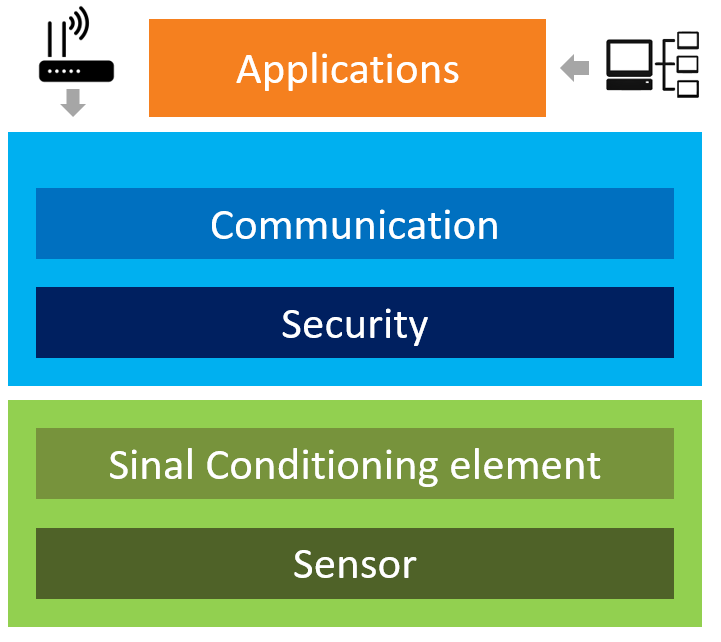
\includegraphics[width=0.3\textwidth]{figs/system-layer.png}
 	\caption{System Layers}
 	\label{System-Layers}
 \end{figure}

The system logic structure is modeled by the use of the knowledge sharing and integration on different domains in the system layers context. This data model, that integrate the contextualized information across the system, is commonly defined on the semantic technologies field as ontology.

In this IoT application, a set of concepts within a domain and the relationships between them is used to perform inference on domain objects. In this concept, the system architecture used here begins with environmental sensing and the inferred information about these data which is relevant for the decision making of the routes, the core of the proposed application.

\subsection{Hardware}

The system hardware consists of a sensing circuit and a routing and processing node implemented by a small single-board computer, a Raspberry Pi. The Raspberry Pi is a series of small single-board computers.

The \autoref{sensor-circuit} shows the complete circuit, with both sensors, required to acquire the data. {\ttfamily Pin7} and  {\ttfamily Pin11} are the Raspberry Pi's respective pin whose software uses to acquire data.

\begin{figure}[!tb]
\begin{center}\begin{circuitikz}
  \draw (0,0) -- (0,2) to [R=10<\kilo\ohm>,*-*] (2,2);
  \draw (0,2) -- (0,3) to [R=10<\kilo\ohm>,*-*] (2,3);
  \draw (0,3) to[short,*-o] (0,5) node[above]{$V_{CC}=3.3V$}; % Power supply
  \draw (0,4) to[short,*-] (1.9,4) -- (1.9,4.5);
  \draw (0,0) to [phR=LDR,*-*](2,0) to [eC,l=10<\micro\farad>,*-*](4,0) -- (4,4) -- (2.2,4) -- (2.2,4.5);
  \draw (4,3.5) to[short,*-] (4.5,3.5) node[ground]{};
  \draw (2,2) -- (2,4.5);
  \draw (2.1,4) -- (2.1,4.5);
  \draw (1.4,5.7) rectangle (2.7,4.5)
    node at(2.05,5.1){DHT11};
   %gpio pins
  \draw (2,0) to[short,*-o] (2,-1) node[right]{Pin11};
  \draw (2,2) to[short,*-o] (2.5,2) node[right]{Pin7};

 \end{circuitikz} \end{center}
\caption{Sensor circuit}
\label{sensor-circuit}
\end{figure}

\subsubsection{DHT11: Humidity and Temperature Sensor}

DHT11 is a humidity and temperature sensor that can read temperatures between 0 and 50$^{\circ}$C and humidity between 20 and 90\%.

The temperature value is measured by a NTC thermistor (Negative Temperature Coefficient-thermistors: the resistance lowers with the increase of the temperature) and the relative humidity through a capacitive sensor \cite{robotics2010dht11}, depicted in Fig. \ref{fig-dht11}.

\subsubsection{Luminosity sensor: LDR (Light Dependent Resistor)}

The LDR has a characteristic that makes its resistance vary according to the environment luminosity. The resistance of the LDR varies inversely to the amount of light incident on it. While the beam of light is falling on it, the LDR offers a very low resistance, and when this beam is cut, its resistance increases \cite{ldr2010manual}. Fig. \ref{fig-ldr} shows the LDR sensor used in this project.

\begin{figure}[h]
\centering

    \begin{subfigure}[b]{0.2\textwidth}
		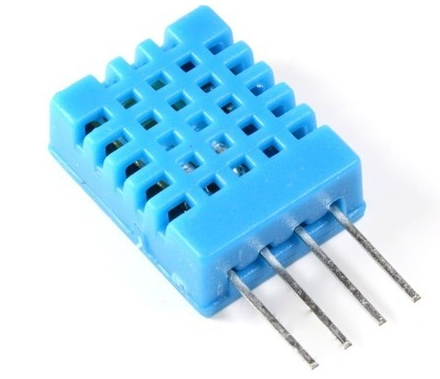
\includegraphics[width=\textwidth]{figs/dht11}
		\caption{DHT11 view}
		\label{fig-dht11}
    \end{subfigure}
    %
    \begin{subfigure}[b]{0.2\textwidth}
	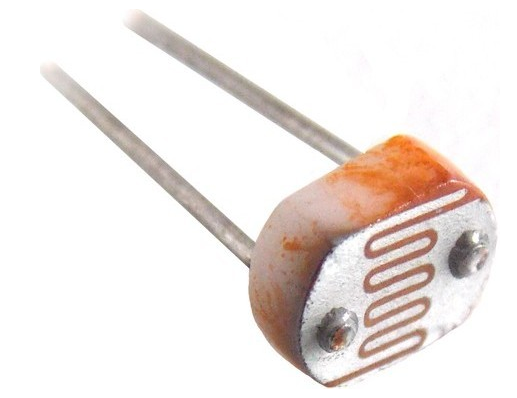
\includegraphics[width=\textwidth]{figs/ldr}
	\caption{LDR sensor}
	\label{fig-ldr}
    \end{subfigure}
	\caption{Sensors}
\end{figure}

%\begin{figure}[tb]
%\centering
%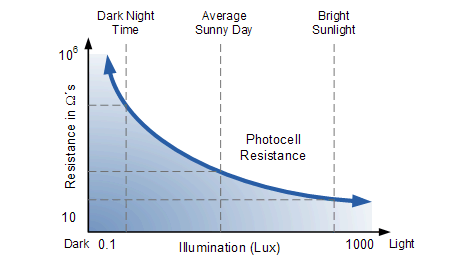
\includegraphics[width=0.5\textwidth]{figs/ldr-2}
%\caption{LDR sensor curve}
%\label{fig-ldr-1}
%\end{figure}
% fonte: http://www.electronics-tutorials.ws/io/io19.gif

\subsection{Software}

The routing context-aware rules follows the sensor information to determine the best route in the network, ensuring the main aim of IoT applications, the objects interconnection.

Initially, the nodes monitor the information coming from the sensing circuit continuously in order to obtain the input parameters to return, as we named in this paper context, their routing condition. This routing condition represents the technical suitability, due to the environmental parameters, so that the node is one of the most apt nodes to integrate the data route. The Fig. \ref{diagram} represents the logical functionality of the proposed system.

The luminosity, humidity and temperature sensors provide the information about the environment conditions. By supplying the context-aware algorithm with the context information, the devices send their sensed data that are compared with pre-determined values in order to be translated as suitable or not suitable to be part of a data route. The flexibility of the algorithm permit that the contribution intensity of each sensor could be changed according to the need and specificity of each context.

\begin{minipage}{.50\textwidth}
\lstinputlisting[language=Python]{codes/pseudo.py}
\end{minipage}

The IoT comprises interconnected objects which are connected to sensors and actuators. The data is collected using sensors, then the sensed information is processed to define the actions. The core of the context-aware routing, as an Internet of Things application, is use the collected information for routing proposes as well. In this aspect, the inference process on the network, the process of using observation and background knowledge as other known premises to determine a conclusion, is extremely important to determine the suitability of the context-aware approach.

% subsection software (end)

% \lipsum[3] %todo: escrever

\begin{figure}[!tb]
\centering
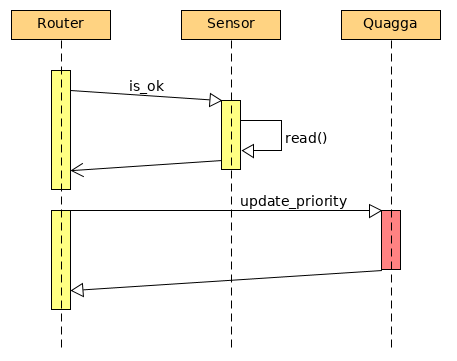
\includegraphics[width=0.38\textwidth]{figs/sequencia}
\caption{Sequence diagram}
\label{diagram}
\end{figure}

% \lipsum[4] %todo: escrever

\section{Results} % (fold)
\label{sec:results}


%% ------------------   Traduzir   ------------------

\begin{figure}[!tbh]
 \begin{center}
   \begin{tikzpicture}
     \begin{axis}[
         width=\linewidth*0.8, % Scale the plot to \linewidth
         grid=major,
         grid style={dashed,gray!30},
         ylabel=Light,
         legend style={at={(0.5,-0.2)},anchor=north},
         x tick label style={rotate=90,anchor=east}
       ]
       \addplot
        % add a plot from table; you select the columns by using the actual name in
        % the .csv file (on top)
        table[x=x,y=light,col sep=comma] {../externos/dados/LDR.csv};
        % \legend{Plot}
     \end{axis}
   \end{tikzpicture}
   \caption{Light read from sensor}
   \label{fig-ldr-data}
 \end{center}
\end{figure}


% \lipsum[5] %todo: escrever

\begin{figure}[!tb]
 \begin{center}
   \begin{tikzpicture}
     \begin{axis}[
         width=\linewidth*0.8, % Scale the plot to \linewidth
         grid=major,
         grid style={dashed,gray!30},
         ylabel=Temperature,
         legend style={at={(0.5,-0.2)},anchor=north},
         x tick label style={rotate=90,anchor=east}
       ]
       \addplot
       table[x=x,y=temperature,col sep=comma] {../externos/dados/DHT.csv};
        % \legend{Plot}
     \end{axis}
   \end{tikzpicture}
   \caption{Temperature read from sensor}
   \label{fig-temp-data}
 \end{center}
\end{figure}

\begin{figure}[!tbh]
 \begin{center}
   \begin{tikzpicture}
     \begin{axis}[
         width=\linewidth*0.8, % Scale the plot to \linewidth
         grid=major,
         grid style={dashed,gray!30},
         ylabel=Humidity,
         legend style={at={(0.5,-0.2)},anchor=north},
         x tick label style={rotate=90,anchor=east}
       ]
       \addplot
       table[x=x,y=humidity,col sep=comma] {../externos/dados/DHT.csv};
        % \legend{Plot}
     \end{axis}
   \end{tikzpicture}
   \caption{Humidity read from sensor}
 \end{center}
\end{figure}

% \lipsum[6] %todo: escrever
